% !Mode:: "TeX:UTF-8"

\begin{frame}{第二十一讲、重积分的计算习题课}
	\linespread{1.5}
	\begin{enumerate}
	  \item {\bf 内容与要求}%{\b (\S 11.4)}
	  \begin{itemize}
		\item 重积分的概念与性质
		\item 重积分的计算
		\item 坐标变换下的重积分
	    \item 重积分的应用
	  \vspace{1em}
	  \end{itemize}
% 	  \item {\bf  课后作业:}
% 	  \begin{itemize}
% 	    \item {\b 习题11.4:1,4,6(2),9,12}
% 	  \end{itemize}
	\end{enumerate}
\end{frame}

\begin{frame}{二重积分的计算}
	\linespread{1.5}\pause 
	\begin{exampleblock}{{\bf 例1:}计算下列二重积分\hfill}\pause 
		\begin{enumerate}
		  \item $\ds\iint_Dxye^{xy^2}\d\sigma,\,D=\{0\leq x\leq 1,0\leq
		  y\leq 1\}$\pause 
		  \item $\ds\iint_D\df 1{x+y}\d\sigma,\,D=\{0\leq x\leq 1,1\leq x+y\leq
		  2\}$\pause 
		  \item $\ds\iint_D|x^2+y^2-4|\d\sigma,\,D=\{x^2+y^2\leq 9\}$\pause 
		  \item $\ds\iint_D(x+y)\mathrm{sgn}(x-y)\d\sigma,\,D=\{0\leq x\leq 1,0\leq
		  y\leq 1\}$
		\end{enumerate}
	\end{exampleblock}
\end{frame}

\begin{frame}{二重积分的积分次序}
	\linespread{1.2}\pause 
	\begin{exampleblock}{{\bf 例2:}改变下列累次积分的次序\hfill}\pause 
		\begin{enumerate}
		  \item $\dint_0^1\dint_0^xf(x,y)\d
		  y\d x+\dint_1^2\dint_0^{2-x}f(x,y)\d y\d x$\pause
		  \item $\dint_0^{2a}\dint_{\sqrt{2ax-x^2}}^{\sqrt{2ax}}
		  f(x,y)\d y\d x,\;(a>0)$\pause 
		  \item $\dint_0^{2\pi}\dint_0^{\sin x}f(x,y)\d y\d x$
		\end{enumerate}
	\end{exampleblock}
\end{frame}

\begin{frame}{二重积分与定积分}
	\linespread{1.2}\pause 
	\begin{exampleblock}{{\bf 例3}\hfill}
		设$f(x)$在区间$[a,b]$连续且恒大于零,证明:
		$$\dint_a^bf(x)\d x\dint_a^b\df{\d x}{f(x)}\geq (b-a)^2$$
	\end{exampleblock}
	\bigskip\pause 
	\begin{exampleblock}{{\bf 例3'}\hfill}
		利用二重积分的方法证明
		$$\left[\dint_a^bf(x)g(x)\d x\right]^2\leq
		\dint_a^bf\,^2(x)\d x\dint_a^bg^2(x)\d x$$
	\end{exampleblock}
\end{frame}

\begin{frame}{二重积分与坐标变换}
	\linespread{1.2}\pause 
	\begin{exampleblock}{{\bf 例4}\hfill}
		计算
		$$\iint_{x^2+y^2\leq 1}\df{\d\sigma}{(x^2+y^2)^m}$$
	\end{exampleblock}\pause 
	\begin{exampleblock}{{\bf 例5}\hfill}
		设$f(x)$可微,$f(0)=0,\,f\,'(0)=1$,求
		$$\lim\limits_{t\to 0^+}\df 1{\pi t^3}
		\iint_{x^2+y^2\leq t^2}f\left(
		\sqrt{x^2+y^2}\right)\d x\d y$$
	\end{exampleblock}
\end{frame}

\begin{frame}{二重积分与坐标变换}
	\linespread{1.2}
	\begin{exampleblock}{{\bf 例6}\hfill}
		计算
		$$\iint_{x^2+4y^2\leq 1}(x^2+y^2)\d\sigma$$
	\end{exampleblock}
	\pause
	\alert{设$x=x(u,v),y=y(u,v)$,\pause 则}
	$$\alert{\iint_Df(x,y)dxdy=\iint_D
	f(x,y)\left|\df{\p(x,y)}{\p(u,v)}\right|
	\d u\d v}$$
\end{frame}

\begin{frame}{二重积分与坐标变换$^*$}
	\linespread{1.2}\pause 
	\begin{exampleblock}{{\bf 例7}}
		通过适当的变量替换,将下列二重积分化为定积分\pause 
		\begin{enumerate}
		  \item $\ds\iint_{|x|+|y|\leq 1}f(x+y)\d\sigma$\pause 
		  \item $\ds\iint_Df(xy)\d\sigma$,$D$由$xy=1,xy=2,y=x$,
		  
		  $y=4x,(x>0,y>0)$围成\pause 
		  \item $\ds\iint_{x^2+y^2\leq 1} f(ax+by+c)\d\sigma,\;(a^2+b^2\ne 0)$
		\end{enumerate}
	\end{exampleblock}
\end{frame}

\begin{frame}{三重积分的计算}
	\linespread{1.2} 
	\begin{exampleblock}{{\bf 例8}\hfill}
		设$f(z)$连续,证明:
		$$\iiint_{x^2+y^2+z^2\leq 1}f(z)\d V=\pi\dint_{-1}^1f(u)(1-u^2)\d u$$
	\end{exampleblock}
	\bigskip\pause
	\begin{exampleblock}{{\bf 例9}\hfill}
		计算三重积分
		$$\iiint_{\Omega}z^2\d V,\;\Omega:x^2+y^2+z^2\leq 1,\,z\geq 0$$
	\end{exampleblock}	
\end{frame}

\begin{frame}{三重积分的积分次序}
	\linespread{1.2}
	\begin{columns}
		\column{.6\textwidth}
			\begin{exampleblock}{{\bf 例10}\hfill}
				按给定的积分次序重写累次积分
				$$\dint_0^1\dint_0^x\dint_0^{xy}f(x,y,z)\d z\d y\d x$$
				\begin{enumerate}
				  \item 先$y$后$z$后$x$
				  \item 先$x$后$z$后$y$
				\end{enumerate}
			\end{exampleblock}
		\column{.4\textwidth}
			\begin{center}
				\pause \resizebox{!}{5cm}{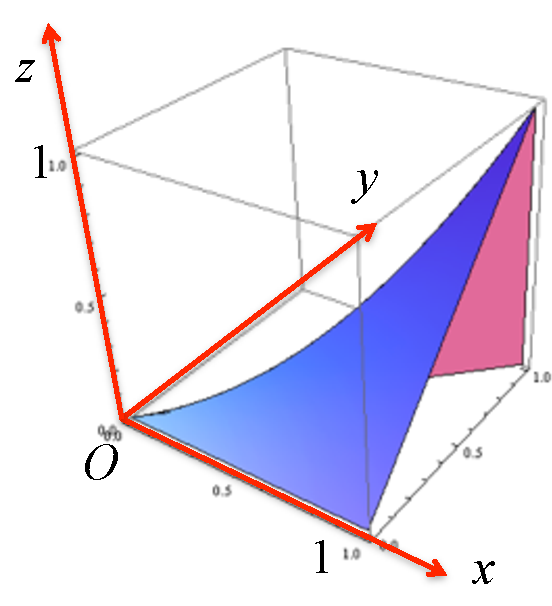
\includegraphics{./images/ch11/xyzC.pdf}}
			\end{center}
	\end{columns}
\end{frame}

\begin{frame}{三重积分与坐标变换}
	\linespread{1.5}\pause
	\begin{exampleblock}{{\bf 例11}\hfill}
		针对给定的积分区域,分别用柱坐标和球坐标将三重积分$\ds\iiint_{\Omega}
		f(x,y,z)\d V$化为累次积分:\pause
		\begin{enumerate}
		  \item $\Omega:\,z\leq\sqrt{4-x^2-y^2},\,3z\geq x^2+y^2$\pause 
		  \item $\Omega:\, z\geq x^2+y^2,\,z\leq x$
		\end{enumerate}
	\end{exampleblock}
\end{frame}

\begin{frame}{三重积分与坐标变换}
	\linespread{1.2}
	\begin{exampleblock}{{\bf 例12}\hfill}
		将三重积分
		$$\dint_0^1\dint_{-\sqrt{y-y^2}}^{\sqrt{y-y^2}}
		\dint_0^{\sqrt{3(x^2+3y^2)}}f\left(
		\sqrt{x^2+y^2+z^2}\right)\d z\d x\d y$$
		分别化为柱坐标和球坐标下的三重积分。
	\end{exampleblock}
\end{frame}

\begin{frame}{三重积分与坐标变换}
	\linespread{1.2}
	\begin{exampleblock}{{\bf 例13}\hfill}
		计算积分
		$$\iiint_{\Omega}(x+y+z)^2\d V,$$
		其中$\Omega:\;\df{x^2}{a^2}+\df{y^2}{b^2}+\df{z^2}{c^2}\leq 1$
	\end{exampleblock}
% 	{\bf 注:}令
% 	$$x=ar\sin\varphi\cos\theta,\,y=br\sin\varphi\sin\theta,\,z=cr\cos\varphi$$
% 	则
% 	$$\alert{\iiint_{\Omega}fdV=abc\iiint_{\Omega}fr^2\sin\varphi drd\varphi
% 	d\theta}$$
\end{frame}

\begin{frame}{三重积分与坐标变换}
	\linespread{1.2}
	\begin{exampleblock}{{\bf 例14}\hfill}
		计算由以下平面所围成的立体体积:
		$$a_ix+b_iy+c_iz=\pm h_i,\;i=1,2,3,$$
		其中:$a_i,b_i,c_i(i=1,2,3)$为常数,且
		$$\Delta=\left|\begin{array}{ccc}
		a_1 & b_1 & c_1\\ a_2 & b_2 & c_2 \\ a_3 & b_3 & c_3
		\end{array}\right|\ne 0$$
	\end{exampleblock}
\end{frame}

% \begin{frame}{三重积分与坐标变换*}
% 	\linespread{1.2}
% 	\begin{exampleblock}{{\bf 例15}\hfill}
% 		求以下曲面在第一卦限中所围立体体积
% 		$$\left(\df xa+\df yb\right)^2+\left(\df zc\right)^2=1,$$
% 		其中$a,b,c>0$。
% 	\end{exampleblock}
% \end{frame}

\begin{frame}{三重积分的计算*}
	\linespread{1.2}
	\begin{exampleblock}{{\bf 例15}\hfill}
		计算极限
		$$\lim\limits_{n\to\infty}\df 1{n^4}\iiint_{r\leq n}[r]\d V,$$
		其中$r=\sqrt{x^2+y^2+z^2}$。
	\end{exampleblock}
	\pause
	$$\alert{\df 43\pi\left[n^4-\sum
	\limits_{k=1}^nk^3\right]}$$
\end{frame}

\begin{frame}{三重积分的计算*}
	\linespread{1.2}
	\begin{exampleblock}{{\bf 例16}\hfill}
		设$f(x)$可微,
		$$F(t)=\iiint_{x^2+y^2+z^2\leq t^2}f(x^2+y^2+z^2)\d V,$$
		求$F\,'(t)$。
	\end{exampleblock}
\end{frame}

\begin{frame}{三重积分的计算*}
	\linespread{1.2}
	\begin{exampleblock}{{\bf 例17}\hfill}
		设$f(x)$可微,
		$$F(x)=\dint_0^x\d v\dint_0^v\d u\dint_0^uf(t)\d t,$$
		求$F\,'(x)$。
	\end{exampleblock}
% 	\pause
% 	$$\alert{\df{x^2}2\dint_0^xf(t)dt-x\dint_0^xtf(t)dt
% 	+\df 12\dint_0^xt^2f(t)dt}$$
\end{frame}

% \begin{frame}{三重积分的计算*}
% 	\linespread{1.2}
% 	\begin{exampleblock}{{\bf 例19}\hfill}
% 		$$I=\iiint_{x^2+y^2+z^2}(x+y+z-10)\d V,$$
% 		证明:
% 		$$28\sqrt 3\pi\leq I\leq 52\sqrt 3\pi$$
% 	\end{exampleblock}
% % 	\pause
% % 	$$\alert{\df{x^2}2\dint_0^xf(t)dt-x\dint_0^xtf(t)dt
% % 	+\df 12\dint_0^xt^2f(t)dt}$$
% \end{frame}

\begin{frame}{重积分的应用}
	\linespread{1.2}
	\begin{exampleblock}{{\bf 例18}\hfill}
		在一半径为$R$的球内,以某条直径为轴打一个半径为$r(r<R)$的
		圆孔,求打孔后球内剩余部分的体积。
	\end{exampleblock}
	\bigskip\pause
	\begin{exampleblock}{{\bf 例19}\hfill}
		求锥面$3(x^2+y^2)=(z-3)^2$与$z=0$所围的内切球面
		与该锥面所围成的立体的体积。
	\end{exampleblock}
\end{frame}

% \begin{frame}{重积分的应用}
% 	\linespread{1.2}
% 	\begin{exampleblock}{{\bf 例22}\hfill}
% 		某火山的表面为曲面
% 		$$z=h\,\mathrm{exp}\left(-\df{\sqrt{x^2+y^2}}{4h}\right),$$
% 		其中$h>0,\,x^2+y^2\leq R^2$。经历一次喷发后,共在火山上落下体积为
% 		$V$的一层等厚度的熔岩,求落下的熔岩厚度。
% 	\end{exampleblock}
% \end{frame}

\begin{frame}{$n$重积分*}
	\linespread{1.2}
	\begin{exampleblock}{{\bf 例20}\hfill}
		求$n$维单纯形
		$$T_n:\; x_i\geq 0\,(i=1,2,\ldots,n),\;
		\sum\limits_{i=1}^nx_i\leq a$$
		的体积$(a>0)$。
	\end{exampleblock}
	\pause
	$$\alert{\df{a^n}{n!}}$$
\end{frame}

\begin{frame}{$n$重积分*}
	\linespread{1.2}
	\begin{exampleblock}{{\bf 例21}\hfill}
		证明:
		$$\dint_0^t\d t_1\dint_0^{t_1}\d t_2\ldots
		\dint_0^{t_{n-1}}\prod\limits_{i=1}^nf(t_i)\d t_n
		=\df 1{n!}\left[\dint_0^tf(s)\d s\right]^n$$
	\end{exampleblock}
\end{frame}

\begin{frame}{$n$重积分*}
	\linespread{1.2}
	\begin{exampleblock}{{\bf 例22}\hfill}
		求$n$维单位球
		$$\sum\limits_{k=1}^nx_k^2\leq 1$$
		的体积。
	\end{exampleblock}
	\pause
	$$\alert{\Gamma(\alpha)=\dint_0^{+\infty}x^{\alpha-1}e^{-x}dx,\;(\alpha>0)}$$
	\pause
	$$\alert{V_n=\df{2\pi^{n/2}}{n\Gamma(n/2)}}$$
\end{frame}

\begin{frame}
	\linespread{1.2}
	\begin{exampleblock}{{\bf 课后练习1}\hfill}
		设$f(x)$在$[a,b]$上单调递增且恒为正,证明
		$${\dint_0^1xf\,^2(x)\d x}{\dint_0^1f(x)\d x}\leq
		{\dint_0^1f\,^2(x)\d x}{\dint_0^1xf(x)\d x}$$
	\end{exampleblock}
	\bigskip
	\begin{exampleblock}{{\bf 课后练习2}\hfill}
		设$a^2+b^2=1,\, D:x^2+y^2\leq 1$,证明
		$$\iint_Df(ax+by)\d x\d y=2\dint_{-1}^1f(u)\sqrt{1-u^2}\d u.$$
	\end{exampleblock}
\end{frame}

\begin{frame}{三重积分与坐标变换*}
	\linespread{1.2}
	\begin{exampleblock}{{\bf 例23}\hfill}
		求以下曲面在第一卦限中所围立体体积
		$$\left(\df xa+\df yb\right)^2+\left(\df zc\right)^2=1,$$
		其中$a,b,c>0$。
	\end{exampleblock}
\end{frame}

%=====================================

% \begin{frame}{title}
% 	\linespread{1.2}
% 	\begin{exampleblock}{{\bf title}\hfill}
% 		123
% 	\end{exampleblock}
% \end{frame}
% 
% \begin{frame}{title}
% 	\linespread{1.2}
% 	\begin{block}{{\bf title}\hfill}
% 		123
% 	\end{block}
% \end{frame}